\subsubsection{Resolver la ecuación del Cohete}

\vspace{0.5cm}

\noindent \textbf{Problema.} The upward velocity of a rocket can be computed by the following formula:

\begin{equation*}
    v = u ln\left(\frac{m_o}{m_o -qt}\right) -gt
\end{equation*}

\noindent where $v = \textnormal{upward velocity} $,  $u = \textnormal{velocity at which fuel is expelled relative to the rocket}$, $m_o = \textnormal{initial mass of the rocket at time} $ $t=0$,  $q = \textnormal{fuel consumption rate}$, and $g = \textnormal{downward acceleration of gravity}$ (assumed constant = $9.8 m/s^2 $). If $u=1800m/s$, $m_o=160000kg$ and $q=2500kg/s$, use six-segment trapezoidal and Simpson's $1/3$ rule, six-point Gauss quadrature, and $O(h^8)$ Romberg mehtods to determine how high the rocket will fly in 30 s.

\begin{itemize}
    \item Solución con Python
\end{itemize}

\begin{figure}[h!]
    \centering
    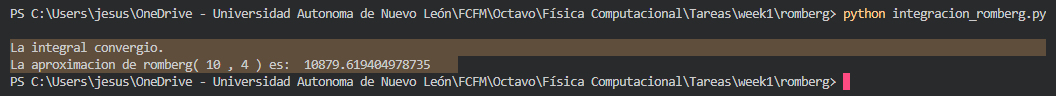
\includegraphics[width=1\linewidth]{images/python.png}
    \caption{Se ejecutó el script de Python que resuelve el problema físico.}
    \label{fig_python}
\end{figure}

\begin{itemize}
    \item Solución con Fortran
\end{itemize}

\begin{figure}[H]
    \centering
    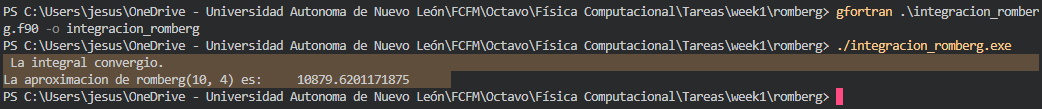
\includegraphics[width=1\linewidth]{images/fortran.png}
    \caption{Se ejecutó el script de Python que resuelve el problema físico.}
    \label{fig_fortran}
\end{figure}

Vea una comparación de las respuestas obtenidas en cada script en la tabla~\ref{table_results}.

\begin{table}[hbt!]
    \begin{threeparttable}
    \caption{Se resolvió el problema de la altura alcanzada por el cohete con el script en Python y Fortran.}
    \label{table_results}
    \begin{tabular}{ll}
    \toprule
    \headrow  & Altura alcanzada en 30 segundos \\
    \midrule
    Python & 10879.61940497 metros \\ 
    \midrule
    Fortran & 10879.62011718 metros \\ 
    \bottomrule
    \end{tabular}
\end{threeparttable}
\end{table}